%%% Econ712: Macroeconomics I
%%% Fall 2020
%%% Danny Edgel
%%%
% Due on Canvas Thursday December 3rd, 11:59pm Central Time
%%%

%%%
%							PREAMBLE
%%%

\documentclass{article}

%%% declare packages
\usepackage{amsmath}
\usepackage{amssymb}
\usepackage{array}
\usepackage{bm}
\usepackage{changepage}
\usepackage{centernot}
\usepackage{graphicx}
\usepackage[shortlabels]{enumitem}
\usepackage{fancyhdr}
	\fancyhf{} % sets both header and footer to nothing
	\renewcommand{\headrulewidth}{0pt}
    \rfoot{Edgel, \thepage}
    \pagestyle{fancy}
	
%%% define shortcuts for set notation
\newcommand{\N}{\mathbb{N}}
\newcommand{\Z}{\mathbb{Z}}
\newcommand{\R}{\mathbb{R}}
\newcommand{\Q}{\mathbb{Q}}
\newcommand{\lmt}{\underset{x\rightarrow\infty}{\text{lim }}}
\newcommand{\neglmt}{\underset{x\rightarrow-\infty}{\text{lim }}}
\newcommand{\zerolmt}{\underset{x\rightarrow 0}{\text{lim }}}
\newcommand{\loge}[1]{\text{ln}\left(#1\right)}
\newcommand{\usmax}[1]{\underset{#1}{\text{max }}}
\newcommand{\Mt}{M_{t+1}^t}
\newcommand{\vhat}{\hat{v}}
\newcommand{\olp}{\overline{p}}
\renewcommand{\L}{\mathcal{L}}
\newcommand{\olq}{\overline{q}}
\newcommand{\zinf}{_{t=0}^\infty}
\newcommand{\aneg}{A^{-1}}
\newcommand{\sneg}{s^{-1}}
\newcommand{\olk}{\overline{k}}
\newcommand{\olc}{\overline{c}}
\newcommand{\olr}{\overline{r}}
\newcommand{\olpi}{\overline{\pi}}
\newcommand{\Aneg}{A^{-1}}
\renewcommand{\sneg}{s^{-1}}
\newcommand{\dc}[1]{\Delta c_{#1}}

\newcommand{\E}[1]{\mathbb{E}\left[#1\right]} % expected value
\newcommand{\Et}[1]{\mathbb{E}_t\left[#1\right]}

%%% define column vector command (from Michael Nattinger)
\newcount\colveccount
\newcommand*\colvec[1]{
        \global\colveccount#1
        \begin{pmatrix}
        \colvecnext
}
\def\colvecnext#1{
        #1
        \global\advance\colveccount-1
        \ifnum\colveccount>0
                \\
                \expandafter\colvecnext
        \else
                \end{pmatrix}
        \fi
}

%%% define function for drawing matrix augmentation lines
\newcommand\aug{\fboxsep=-\fboxrule\!\!\!\fbox{\strut}\!\!\!}

\makeatletter
\let\amsmath@bigm\bigm

\renewcommand{\bigm}[1]{%
  \ifcsname fenced@\string#1\endcsname
    \expandafter\@firstoftwo
  \else
    \expandafter\@secondoftwo
  \fi
  {\expandafter\amsmath@bigm\csname fenced@\string#1\endcsname}%
  {\amsmath@bigm#1}%
}


%________________________________________________________________%

\begin{document}

\title{	Problem Set \#3 }
\author{ 	Danny Edgel 					\\ 
			Econ 712: Macroeconomics I		\\
			Fall 2020						\\
		}
\maketitle\thispagestyle{empty}

%%%________________________________________________________________%%%

\noindent\textit{Collaborated with Sarah Bass, Emily Case, Michael Nattinger, and Alex Von Hafften}

%%%________________________________________________________________%%%
\subsection*{Question 1}

\begin{enumerate}[(a)]
	\item 
	
	\item 
	
	
	\item 
	
	
	\item 
	
	
	\item 
	
	
\end{enumerate}

%%%________________________________________________________________%%%
\subsection*{Question 2}

\begin{enumerate}[(a)]
	\item A recurisve competitive equilibrium is a continuous pricing function, $p(x)$, and a continuous, bounded value function, $V(a,x)$, such that:
		\begin{enumerate}[(i)]
			\item $V(a,x)$ solves the Bellman equation 
			\item $\forall x$, $V(a,x)$ is attained by $c=x$, $x'=1$
		\end{enumerate}
	
	\item The stochastic endowment in this model, $x_t$, is the dividend. In equilibrium, ${p_t = \E{\beta\frac{u'(c_{t+1})}{u(c_t)}(p_{t+1}+x_{t+1})}}$ where ${c_t=x_t}$ and ${x_{t+1}=1}$. Thus, with logarithmic utility and using a Taylor expansion around ${\dc{t+1}=0}$ and ${p_{t+1}=}$, we can solve:
		\begin{align*}
			p_t 			&= \Et{\beta\frac{c_t}{c_{t+1}}(p_{t+1}+x_{t+1})}			\\
							&= \Et{\beta\frac{1}{1+\dc{t+1}}(p_{t+1}+1)}				\\
			\frac{p_t}{x_t}	&= \frac{1}{x_t}\Et{\beta\frac{1}{1+\dc{t+1}}(p_{t+1}+1)}	\\
		\end{align*}
	
	
	\item 
	
	
	\item 
	
	
\end{enumerate}

%%%________________________________________________________________%%%
\subsection*{Question 3}

\begin{enumerate}[(a)]
	\item The Bellman equation for the consumer's problem is:
		\[
			V(a,l) = \usmax{a}\left\{\frac{c^{1-\gamma}}{1-\gamma} + \beta\E{V(a',l')}\right\}\text{ s.t. } c + a' \leq wl + (1+r)a 
		\]
		Since the consumer does not value leisure, the budget constraint will hold with equality, and the Bellman becomes:
		\[
			V(a,l) = \usmax{a}\left\{\frac{(wl + (1+r)a - a')^{1-\gamma}}{1-\gamma} + \beta\int V(a',l')Q(l,dl')\right\}
		\]
		We can find the optimality conditions by taking the first order condition of the maximization problem and using the envelope condition:
		\begin{eqnarray*}
			\left(wl + (1+r)a - a'\right)^{-\gamma}(1+r) + \beta\int V'(a',l')Q(l,dl') = 0	\\
			V'(a',l') = \left(wl' + (1+r)a' - a''\right)^{-\gamma}(-1)	\\
			\left(wl + (1+r)a - a'\right)^{-\gamma}(1+r) = \beta\E{\left(wl' + (1+r)a' - a''\right)^{-\gamma}}
		\end{eqnarray*}
	
	\item We can find the stationary distribution of the labor endowment by choosing an arbitrary starting point, $l_0$, for the labor endowment, where $l_0$ is a row vector with one entry equal to one and the other equal to 0, then iteratively calculating ${l=l_0Q}$, setting ${l_0=l}$, then repeating until $l$ converges to an unconditional probability of each labor value. This is done in the attached Matlab code, which outputs ${l=\left[0.25\text{ }0.75\right]}$, where 0.25 is the probability mass of ${l_t=0.7}$, and 0.75 is the probability mass of ${l_t=1.1}$. The unconditional mean, then, is:
		\[
			\E{l_t} = 0.25(0.7) + 0.75(1.1) = 1
		\]
	
	
	\item The attached Matlab file conducts all of the necessary calculations for this problem.
		\begin{enumerate}[i.]
			\item The chart below plots the value function, separated by labor states, against the asset values in the asset grid. The functions appear to be constistent with out assumptions: continuous, concave, differentiable, and strictly increasing. Futhermore, they appear as expected: at every level of asset holdings, the value function is lower for the lower labor supply state than for the higher labor supply state. It is also intuitive that the value function is steeper with respect to asset holdings in the lower labor supply state, as the consumer saves in order to smooth consumption from the high labor supply state to the low labor supply state.
				\begin{center}
					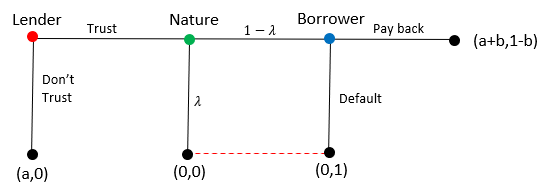
\includegraphics[scale=.75]{figure1.png}
				\end{center}
			
			\item The policy functions, ${a'(a,l_i)}$ are displayed below. There does appear to be a ${\overline{a}\approx 2.175}$ such that ${\forall a\geq\overline{a},a'(a,l_2)<a}$, which is indicated on the chart. The existence of this value and the fact that ${a'(a,l_1)<a}$ for all $a$ suggest that the long-run value of $a_t$ never exceeds $\overline{a}$.
				\begin{center}
					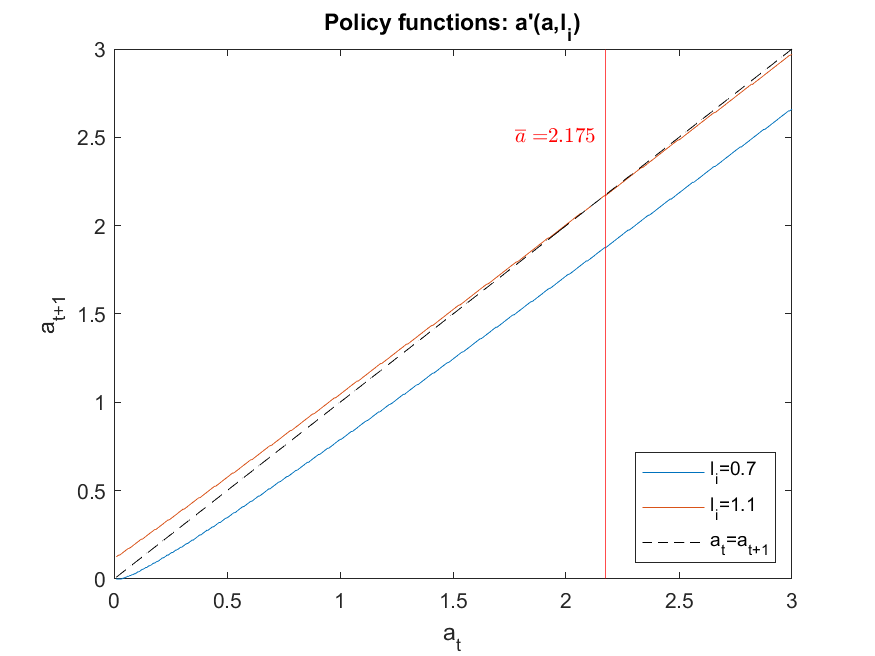
\includegraphics[scale=.75]{figure2.png}
				\end{center}
			
		\end{enumerate}
	
	
	\item The chart below displays the marginal probability mass function for $a_t$, along with its mean, which is ${\approx 1.02}$
		\begin{center}
			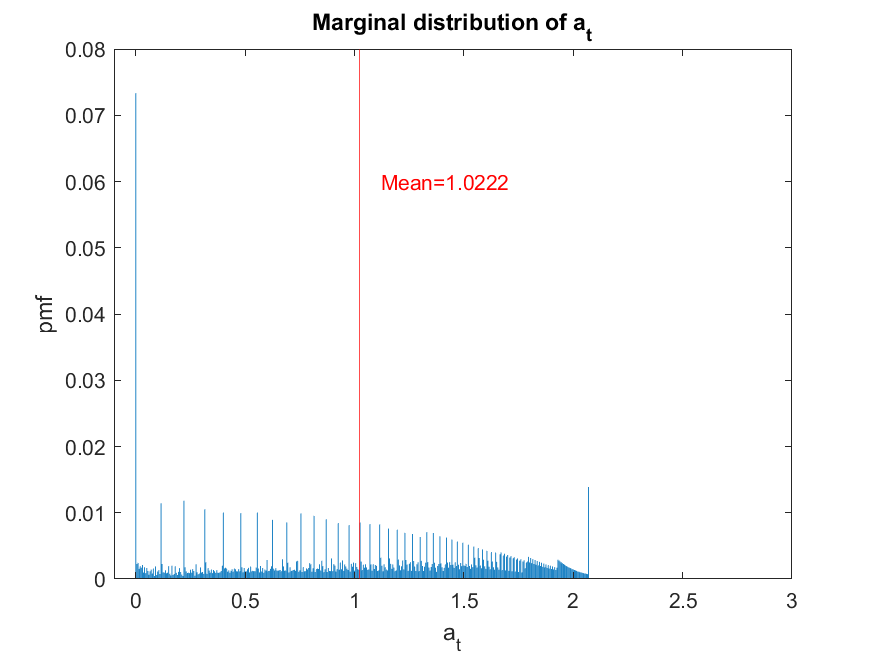
\includegraphics[scale=.75]{figure3.png}
		\end{center}
	
	
\end{enumerate}

%%%________________________________________________________________%%%


\end{document}












